\section{Time synchronization}

Clocks must be synchronized to correlate events from different sensor nodes,
support synchronized sleep cycles, enable localization, ...

\begin{description}
		\item[Clock skew] Difference between reading of two clocks
		\item[Clock drift] Difference between reading of a clock and reference
				clock, per unit of time of reference clock
		\item[Send time] Time needed by packet from application to MAC layer,
				variable because of software delays.
		\item[Access time] Delay due to MAC protocol
		\item[Transmission time] Delay caused by bit transmission, follows from packet length and radio bandwith, deterministic
		\item[Propagation time] Signal propagation, follows from distance and speed of radio waves
		\item[Reception time] Time required to receive bits, deterministic
		\item[Receive time] Processing between MAC and application layer, variable
\end{description}

If drifts $d_{i, j}$ and initial offsets $o_{i, j}$ of two clocks are known,
then:
\begin{align*}
		c_i(t) & = d_i \cdot t + o_i \\
		c_j(t) & = d_j \cdot t + o_i
\end{align*}

Clock times can then be translated between two nodes:
\begin{align*}
		c_i(t) = a_{i, j} \cdot c_j(t) + b_{i, j}
\end{align*}

Where $a_{i, j}:= \frac{d_i}{d_j}$ and $b_{i, j} := - o_i \cdot a_i + o_{j, j}$.

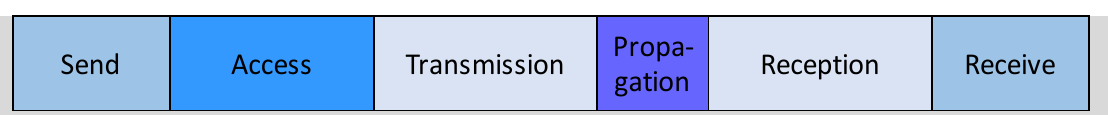
\includegraphics[width=\textwidth]{05_packet_delay}

\subsection{Classification of synchronization}

\begin{description}
		\item[Internal vs external synchronization] Synchronization among nodes vs with external master
		\item[Scope] All nodes vs subset
		\item[Rate vs offset synchronization] what is synchronized
		\item[Time-scale transformation vs clock synchronization] sync clocks or scale local time
		\item[Lifetime] Continuous vs on-demand
\end{description}

Synchronization schemes must be efficient (computational resources, energy,
..), precise, scalable, robust.

\subsection{GPS}

Requires line-of-sight. High power consumption of receiver. Requires four satellites.

\subsection{Time signals}

Time signals by dedicated radio stations. Low power consumption
(\SI{0.266}{\milli\watt} for \SI{1}{\hertz} receiver), error of
\SI{1}{\milli\second} with \SI{500}{\second} update interval on TelosB.

\subsection{Unidirectional synchronization}

Time-stamping of messages. Receiving node knows sending time of sender and
receiving time. Estimates delay $d$ as difference of the two.

\subsection{Roundtrip synchronization}

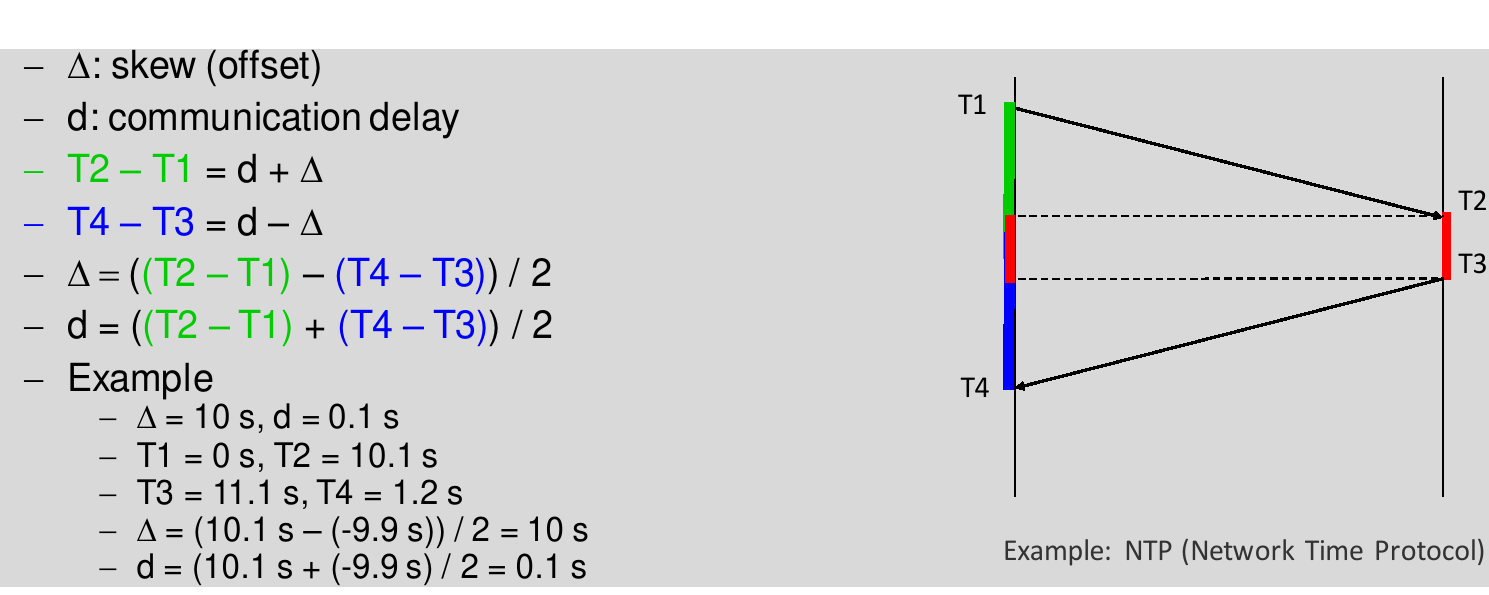
\includegraphics[width=\textwidth]{05_rt_sync}

\subsection{Reference broadcasting}

Can be used when master reaches two nodes, which cannot synchronize with each other.

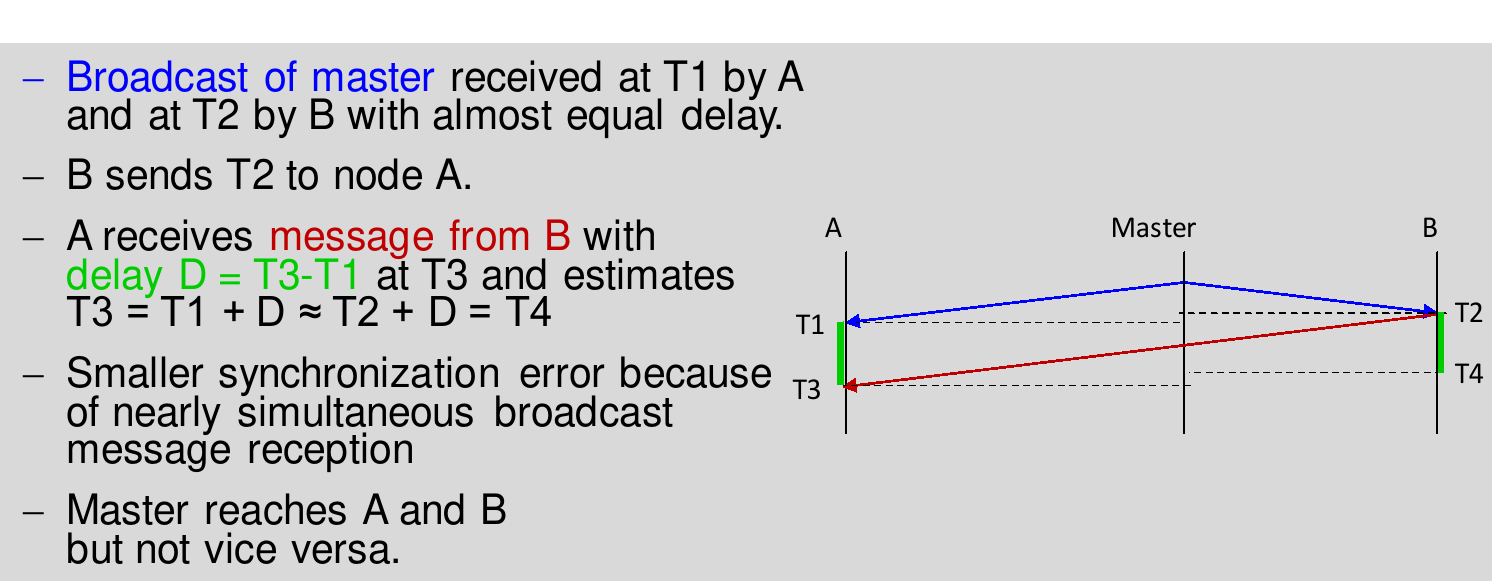
\includegraphics[width=\textwidth]{05_reference_broadcasting}

\subsection{Combining estimates}

Results of multiple synchronizations with same node can be combined using e.g.
linear regreission. Problem: Large memory requirements. Other approaches (e.g.
tiny-sync) more efficient although less accurate.

\subsection{Structured approaches}

Typically multiple nodes need to be synchronized which cannot communicate directly.

\subsubsection{Out-of-band synchronization}

Each node connected to at least one master which is synced to external system, eg GPS.

\subsubsection{Clustering}

All members of cluster can synchronize via e.g. reference broadcasting. Time
gateways (at least one per cluster) translate time stamps between clusters they
are part of. Tradeoff many translations vs large clusters (high power
consumption because of transmission range).

\paragraph{RBS}

Nodes send periodic beacons (pulses). Time difference between events and pulses
can be used to establish relationships.

\paragraph{Time routing in multi-hop networks with RBS}
Single time-gateways not desireable. Instead, dynamic time route establishment.
Each node converts time relationships before sending it on.

\subsubsection{Tree construction}

Synchronization tree with master as root. Single-hop synchronization along
tree. Accuracy degrades with distance from root.

\subsection{Unstructured approaches}

No structure established, completely localized solution.

\subsubsection{Diffusion-based synchronization}

Repeatedly perform steps which will eventually converge to shared time.k

\paragraph{Rate-based synchronous diffusion}

Random diffusion rates per pair of nodes, with sum $< 1$. Exchange time with
all neighbouring nodes. For each neighbour, adjust own time by delta with
neighbour, multiplied with rate: $c_i := c_i + r_{i, j} \cdot (c_j - c_i)$

\paragraph{Asynchronous diffusion}

Ask clock readings from set of random neighbours. Average readings (and use as
own?).  Send new value to neighbours.
